% System Architecture Diagram
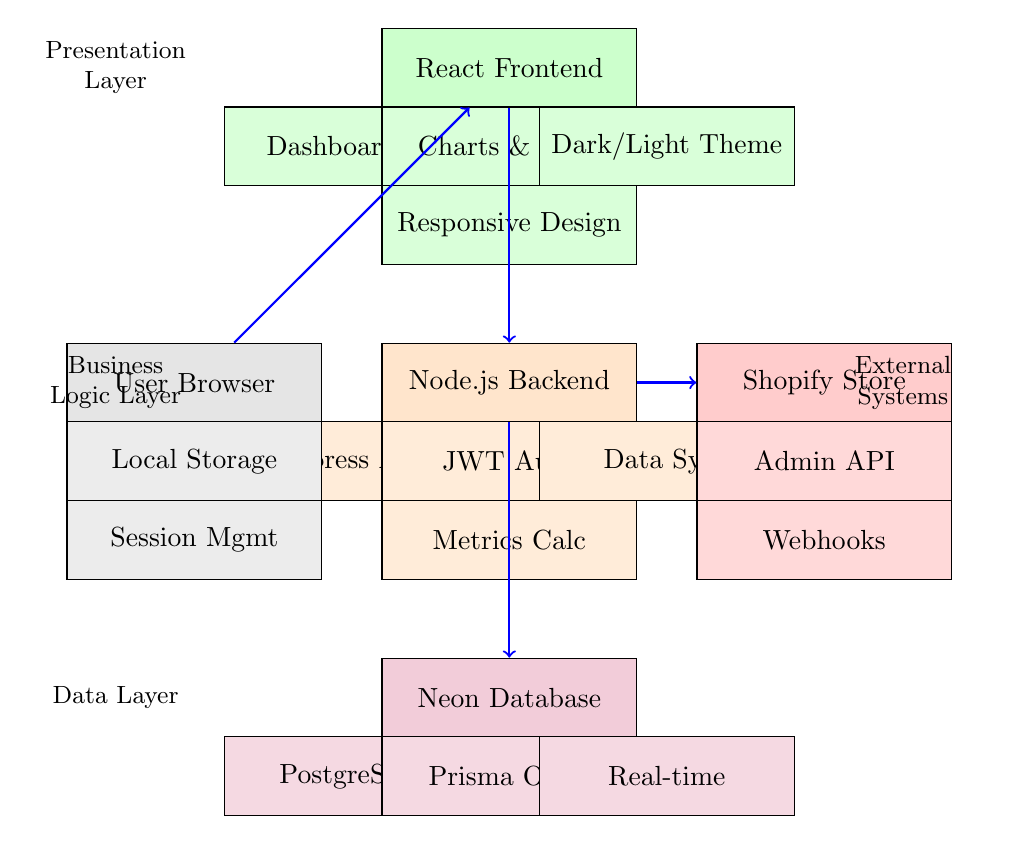
\begin{tikzpicture}[
    node distance=1.5cm,
    box/.style={rectangle, draw, fill=blue!20, text width=3cm, text centered, minimum height=1cm},
    arrow/.style={->, thick, blue},
    label/.style={text width=2cm, text centered, font=\small}
]

% Frontend Layer
\node[box, fill=green!20] (frontend) at (0, 6) {React Frontend};
\node[box, fill=green!15] (ui) at (-2, 5) {Dashboard UI};
\node[box, fill=green!15] (charts) at (0, 5) {Charts \& KPIs};
\node[box, fill=green!15] (theme) at (2, 5) {Dark/Light Theme};
\node[box, fill=green!15] (responsive) at (0, 4) {Responsive Design};

% Backend Layer
\node[box, fill=orange!20] (backend) at (0, 2) {Node.js Backend};
\node[box, fill=orange!15] (api) at (-2, 1) {Express API};
\node[box, fill=orange!15] (auth) at (0, 1) {JWT Auth};
\node[box, fill=orange!15] (sync) at (2, 1) {Data Sync};
\node[box, fill=orange!15] (metrics) at (0, 0) {Metrics Calc};

% Database Layer
\node[box, fill=purple!20] (database) at (0, -2) {Neon Database};
\node[box, fill=purple!15] (postgres) at (-2, -3) {PostgreSQL};
\node[box, fill=purple!15] (prisma) at (0, -3) {Prisma ORM};
\node[box, fill=purple!15] (realtime) at (2, -3) {Real-time};

% External Systems
\node[box, fill=red!20] (shopify) at (4, 2) {Shopify Store};
\node[box, fill=red!15] (adminapi) at (4, 1) {Admin API};
\node[box, fill=red!15] (webhooks) at (4, 0) {Webhooks};

% User
\node[box, fill=gray!20] (user) at (-4, 2) {User Browser};
\node[box, fill=gray!15] (storage) at (-4, 1) {Local Storage};
\node[box, fill=gray!15] (session) at (-4, 0) {Session Mgmt};

% Connections
\draw[arrow] (frontend) -- (backend);
\draw[arrow] (backend) -- (database);
\draw[arrow] (user) -- (frontend);
\draw[arrow] (backend) -- (shopify);

% Layer labels
\node[label] at (-5, 6) {Presentation Layer};
\node[label] at (-5, 2) {Business Logic Layer};
\node[label] at (-5, -2) {Data Layer};
\node[label] at (5, 2) {External Systems};

\end{tikzpicture}
